\section{Experimental results}

%%%%%%%%%%%%%%%%%%%%%%%%%%%%%%%%%%%%%%%%%%%%%%%%%%%%%%%%%%%%%%%%%%%%%%%%%%%%
\begin{frame}{Experimental setup}
    \begin{minipage}[c]{0.7\linewidth}
        \begin{block}{}
            \begin{itemize}
                \item Use of FISSA for FIA campaigns
                \item More complex fault models: multi-bit faults or multi single-bit faults
            \end{itemize}
        \end{block}
    \end{minipage}\hfill%
    \begin{minipage}[c]{0.3\linewidth}
        \begin{figure}
            \centering
            
\includegraphics[width=.75\textwidth]{src/5_results/img/experimental.png}
        \end{figure}
    \end{minipage}
\end{frame}
%%%%%%%%%%%%%%%%%%%%%%%%%%%%%%%%%%%%%%%%%%%%%%%%%%%%%%%%%%%%%%%%%%%%%%%%%%%%
\begin{frame}{Fault model}
    \begin{block}{}
        \begin{itemize}
            \item DIFT-related registers + protection-related registers
            \item Single bit-flip in two registers at two distinct clock cycles% -> 1 fault / clock cycle
            \item Single bit-flip in two registers at a given clock cycle% -> 2 faults / clock cycle
            \item Multi-bit faults in one register at a given clock cycle% -> 6 faults / clock cycle
            \item \underline{Multi-bit faults in two registers at a given clock cycle} {\tiny (registers from 1 to 10 bits only)}% -> 11 faults / clock cycle
        \end{itemize}
    \end{block}
\end{frame}
%%%%%%%%%%%%%%%%%%%%%%%%%%%%%%%%%%%%%%%%%%%%%%%%%%%%%%%%%%%%%%%%%%%%%%%%%%%%%%%%%%%%%%%%%%%%%%%%%%%%%%%%%%%%
\begin{frame}{FPGA implementation results}
    \onslide<1>{
    \begin{table}[t]
        \centering
        \footnotesize
        \caption{FPGA implementation results — Vivado 2023.2}
        \label{tab:chap6_implementation}
        \begin{tabular}{@{}rccc@{}}
            \toprule
            \tableCentered{Protection} & Number of LUTs                                     & Number of FFs                                      & Maximum frequency                        \\ \midrule
            D-RI5CY                    & \num{6911} {\tiny (0\%)   }                        & \num{2335} {\tiny (0\%)   }                        & \SI{47.6}{\mega\hertz} {\tiny (0\%)    } \\
            Simple parity              & \num{7011} {\tiny (1.45\%)}                        & \num{2337} {\tiny (0.09\%)}                        & \SI{47.6}{\mega\hertz} {\tiny (0\%)    } \\
            Hamming Code Strategy 1    & \num{7283} {\tiny (5.38\%)}                        & \textcolor{LimeGreen}{\num{2361} {\tiny (1.11\%)}} & \SI{47.4}{\mega\hertz} {\tiny (-0.36\%)} \\
            Hamming Code Strategy 2    & \textcolor{red}{\num{7369} {\tiny (6.63\%)}}       & \num{2363} {\tiny (1.2\%) }                        & \SI{46.9}{\mega\hertz} {\tiny (-1.43\%)} \\
            Hamming Code Strategy 3    & \num{7251} {\tiny (4.92\%)}                        & \num{2361} {\tiny (1.11\%)}                        & \SI{46.8}{\mega\hertz} {\tiny (-1.67\%)} \\
            Hamming Code Strategy 4    & \num{7203} {\tiny (4.23\%)}                        & \num{2371} {\tiny (1.54\%)}                        & \SI{47.6}{\mega\hertz} {\tiny (0\%)    } \\
            Hamming Code Strategy 5    & \textcolor{LimeGreen}{\num{7182} {\tiny (3.92\%)}} & \textcolor{red}{\num{2411} {\tiny (3.25\%)}}       & \SI{47.3}{\mega\hertz} {\tiny (-0.57\%)} \\
            SECDED Strategy 1          & \num{7428} {\tiny (7.48\%)}                        & \num{2366} {\tiny (1.33\%)}                        & \SI{47.2}{\mega\hertz} {\tiny (-0.95\%)} \\
            SECDED Strategy 2          & \textcolor{red}{\num{7433} {\tiny (7.55\%)}}       & \num{2366} {\tiny (1.41\%)}                        & \SI{47.2}{\mega\hertz} {\tiny (-0.95\%)} \\
            SECDED Strategy 3          & \num{7324} {\tiny (5.98\%)}                        & \textcolor{LimeGreen}{\num{2368} {\tiny (1.28\%)}} & \SI{47.5}{\mega\hertz} {\tiny (-0.24\%)} \\
            SECDED Strategy 4          & \num{7255} {\tiny (4.98\%)}                        & \num{2365} {\tiny (1.93\%)}                        & \SI{48.3}{\mega\hertz} {\tiny (1.43\%) } \\
            SECDED Strategy 5          & \textcolor{LimeGreen}{\num{7228} {\tiny (4.59\%)}} & \textcolor{red}{\num{2428} {\tiny (3.98\%)}}       & \SI{48.3}{\mega\hertz} {\tiny (1.43\%) } \\
            \bottomrule
        \end{tabular}
    \end{table}
    }

    \only<2>{
        \begin{columns}
            \begin{column}{.25\linewidth}
                \hfill
            \end{column}
            \begin{column}{.5\linewidth}
                \begin{alertblock}{}
                    \centering
                    \textcolor{red}{\Forward}~No major impact on area and performances~\textcolor{red}{\Rewind} 
                \end{alertblock}
            \end{column}
            \begin{column}{.25\linewidth}
                \hfill
            \end{column}
        \end{columns}
    }
\end{frame}
%%%%%%%%%%%%%%%%%%%%%%%%%%%%%%%%%%%%%%%%%%%%%%%%%%%%%%%%%%%%%%%%%%%%%%%%%%%%%%%%%%%%%%%%%%%%%%%%%%%%%%%%%%%%
\begin{frame}{Obtained results from the considered fault model}
    \begin{table}[H]
        \centering
        \footnotesize
        \caption{Logical fault injection simulation campaigns results for exhaustive multi-bits faults in two registers at a given clock cycle}
        \label{tab:chap6_results_multi_bitflip_reg_multi}
        \setlength{\tabcolsep}{2pt}
        \begin{tabular}{@{}ccccccccccc@{}}
            \toprule
                                                               &               & Crash & Silent       & Delay & Detection   & \tableTwoLines{Detection \&}{Correction} & \tableTwoLines{Double Error}{Detection} & Success                                      & Total        & \tableTwoLines{Execution}{time (h:min)} \\\midrule
            \multirow{12}{*}{\tableTwoLines{Buffer}{Overflow}} & No protection & 0     & \num{67072 } & 926   & --          & --                                       & --                                      & \textcolor{blue}{450 {\tiny (0.66\%)}}  & \num{68448 } & 11:11                                   \\
                                                               & Simple parity & 0     & \num{24622 } & 8     & \num{53359} & --                                       & --                                      & 59 {\tiny (0.08\%)}                          & \num{78048 } & 25:00                                   \\
                                                               & Hamming 1     & 0     & \num{294464} & 6273  & --          & --                                       & --                                      & 3103 {\tiny (1.02\%)}                        & \num{303840} & 99:36                                   \\
                                                               & Hamming 2     & 0     & 0            & 3992  & --          & \num{319588}                             & --                                      & \textcolor{red}{4356 {\tiny (1.33\%)}} & \num{327936} & 131:12                                  \\
                                                               & Hamming 3     & 0     & 0            & 4557  & --          & \num{436187}                             & --                                      & 4408 {\tiny (0.99\%)}                        & \num{445152} & 121:20                                  \\
                                                               & Hamming 4     & 0     & 0            & 5446  & --          & \num{590953}                             & --                                      & 5329 {\tiny (0.89\%)}                        & \num{601728} & 167:00                                  \\
                                                               & Hamming 5     & 0     & 0            & 5987  & --          & \num{714873}                             & --                                      & 5860 {\tiny (0.81\%)}                        & \num{726720} & 210:31                                  \\
                                                               & SECDED 1      & 0     & 0            & 1911  & --          & \num{150791}                             & \num{170575}                            & 723 {\tiny (0.22\%)}                         & \num{324000} & 86:59                                   \\
                                                               & SECDED 2      & 0     & 0            & 1186  & --          & \num{170805}                             & \num{184761}                            & 584 {\tiny (0.16\%)}                         & \num{357336} & 94:04                                   \\
                                                               & SECDED 3      & 0     & 0            & 1230  & --          & \num{300260}                             & \num{263665}                            & 669 {\tiny (0.12\%)}                         & \num{565824} & 161:30                                  \\
                                                               & SECDED 4      & 0     & 0            & 18    & --          & \num{457498}                             & \num{368959}                            & 61 {\tiny (0.01\%)}                          & \num{826536} & 244:48                                  \\
                                                               & SECDED 5      & 0     & 0            & 39    & --          & \num{576992}                             & \num{401407}                            & \textcolor{LimeGreen}{66 {\tiny (0.01\%)}}   & \num{978504} & 284:45                                  \\
            \bottomrule
        \end{tabular}
    \end{table}
\end{frame}
%%%%%%%%%%%%%%%%%%%%%%%%%%%%%%%%%%%%%%%%%%%%%%%%%%%%%%%%%%%%%%%%%%%%%%%%%%%%%%%%%%%%%%%%%%%%%%%%%%%%%%%%%%%%
\begin{frame}{Generated heatmaps from FISSA with the current fault model}
    \begin{figure}
        \centering
        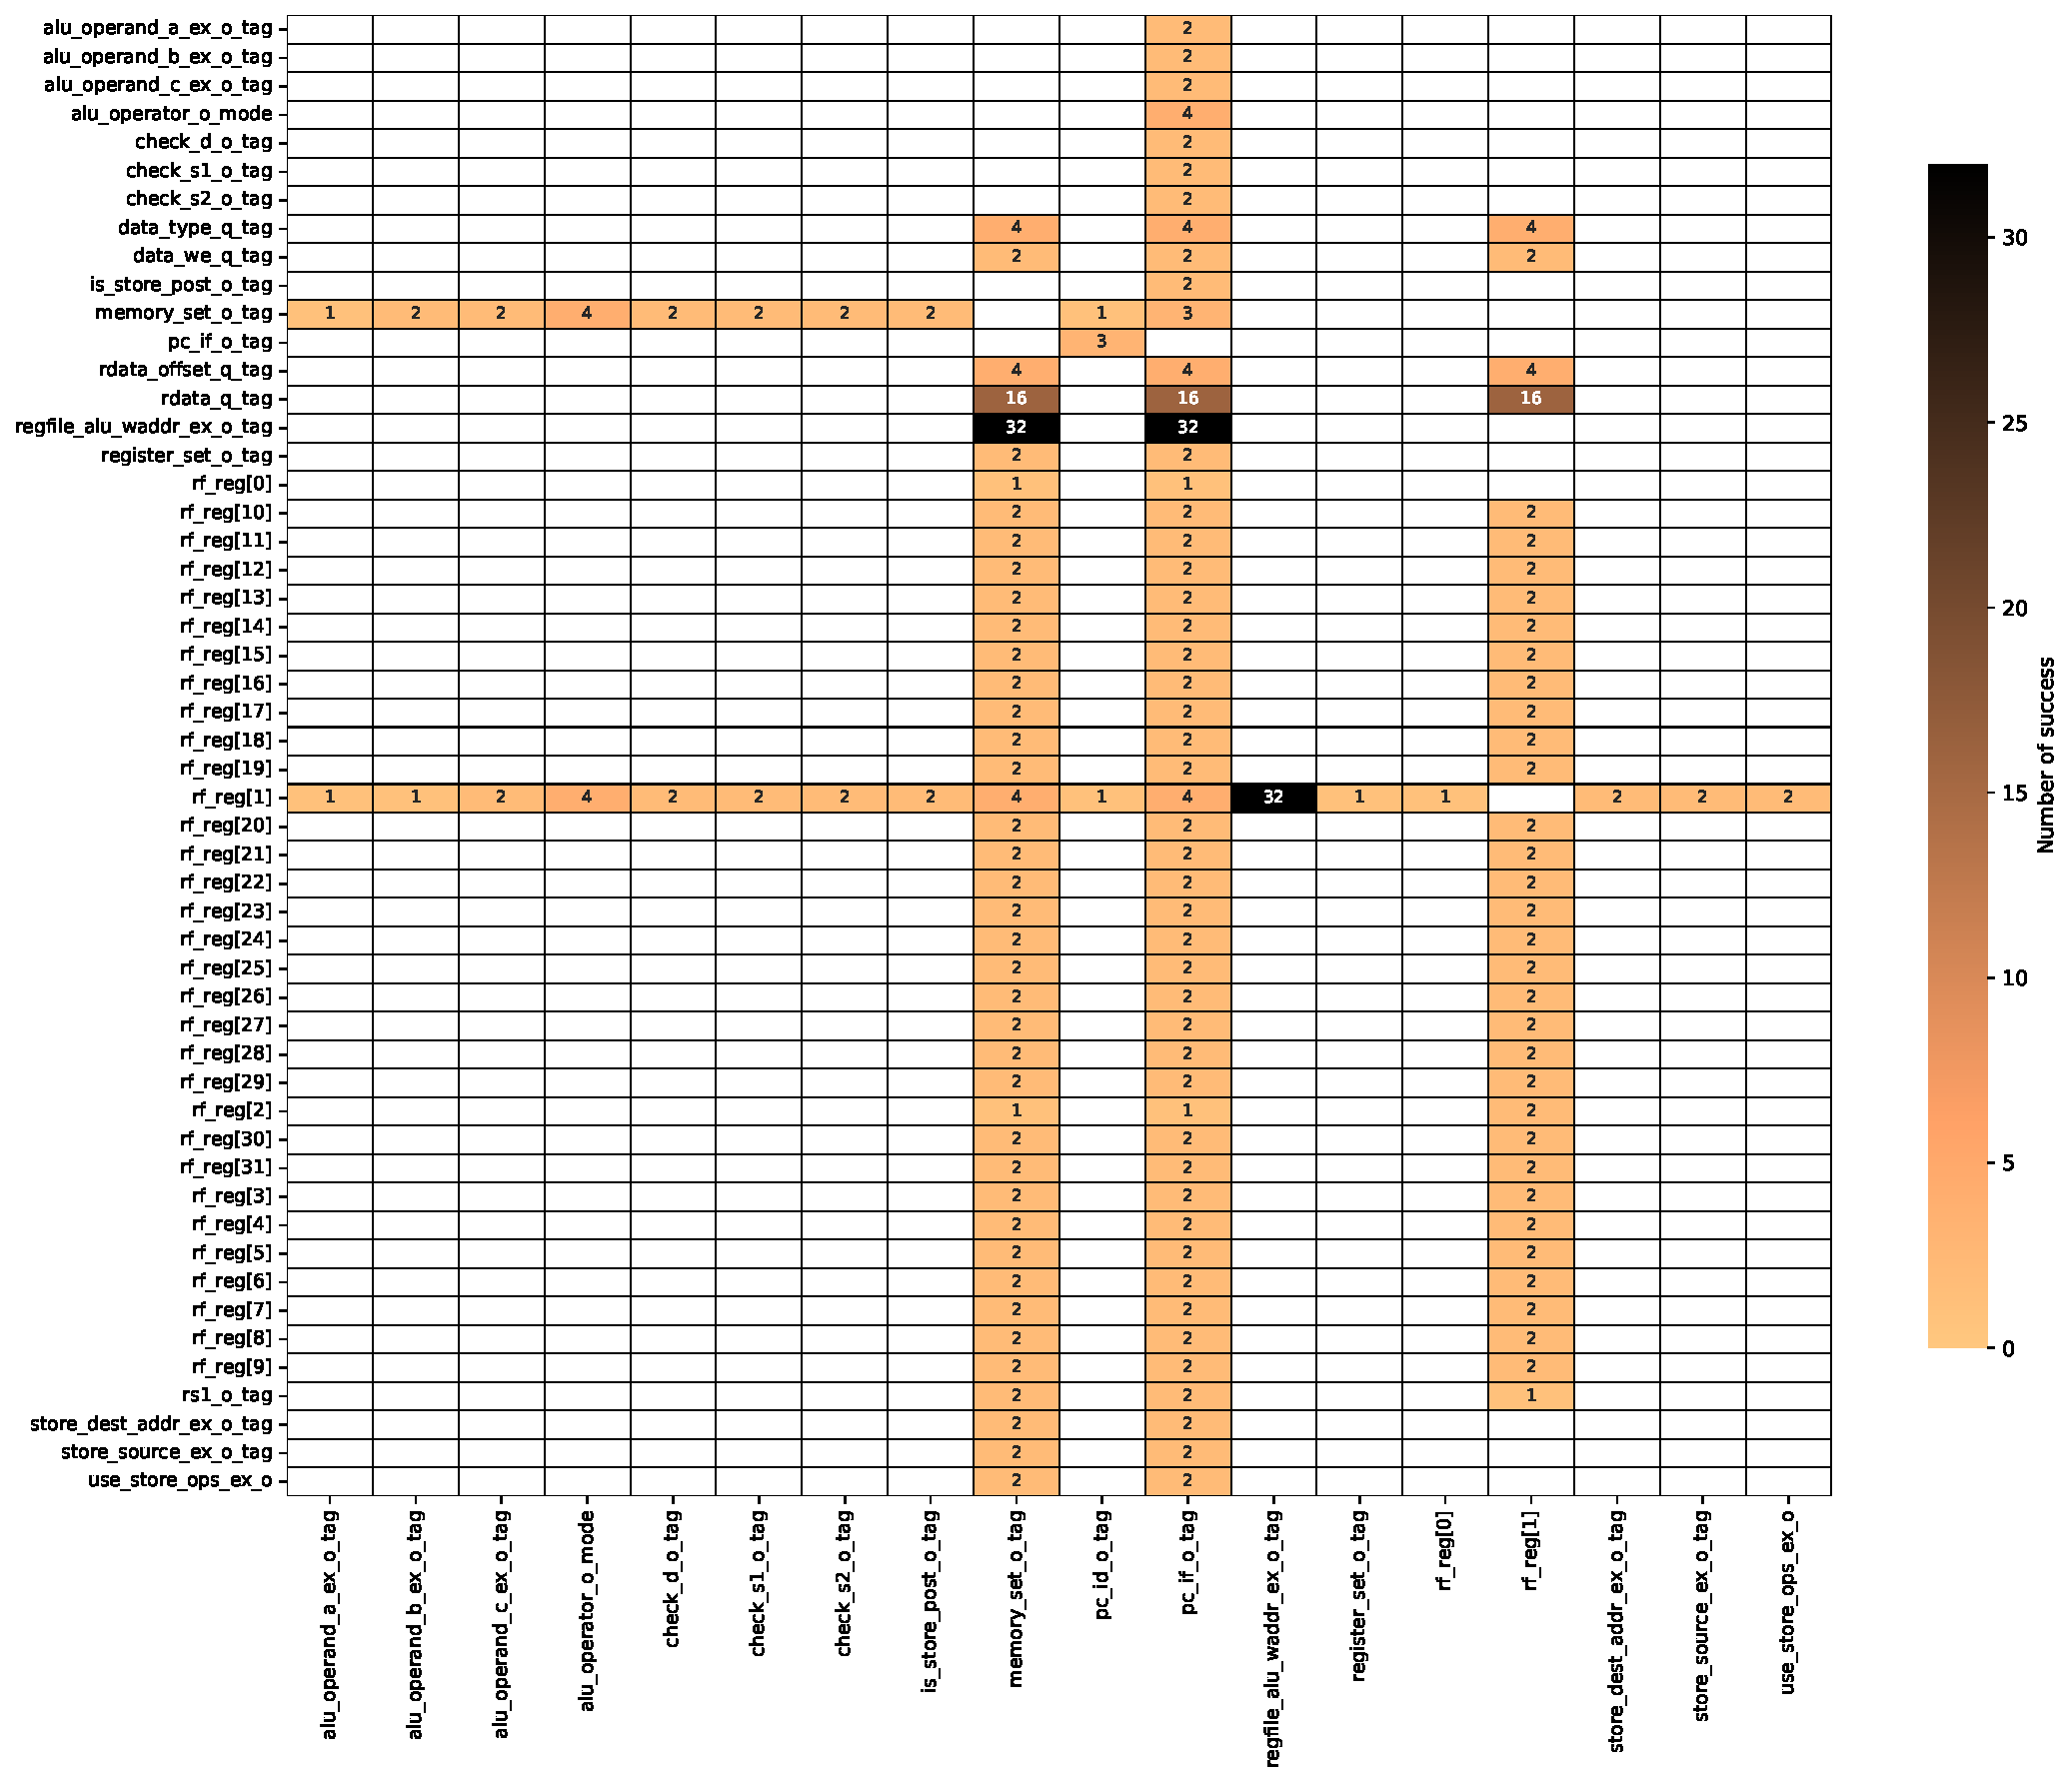
\includegraphics[height=.825\textheight]{src/5_results/img/heatmap_buffer_overflow_wop_1_multi_bitflip_reg_multi_2.pdf}
        \caption{Unprotected version: multi-bits faults in two registers at a given clock cycle $\rightarrow$ 450 successes}
        \label{fig:heatmap_multibit_1}
    \end{figure}
\end{frame}

\begin{frame}{}
    \begin{minipage}[c]{0.45\linewidth}
        \begin{figure}
            \centering
            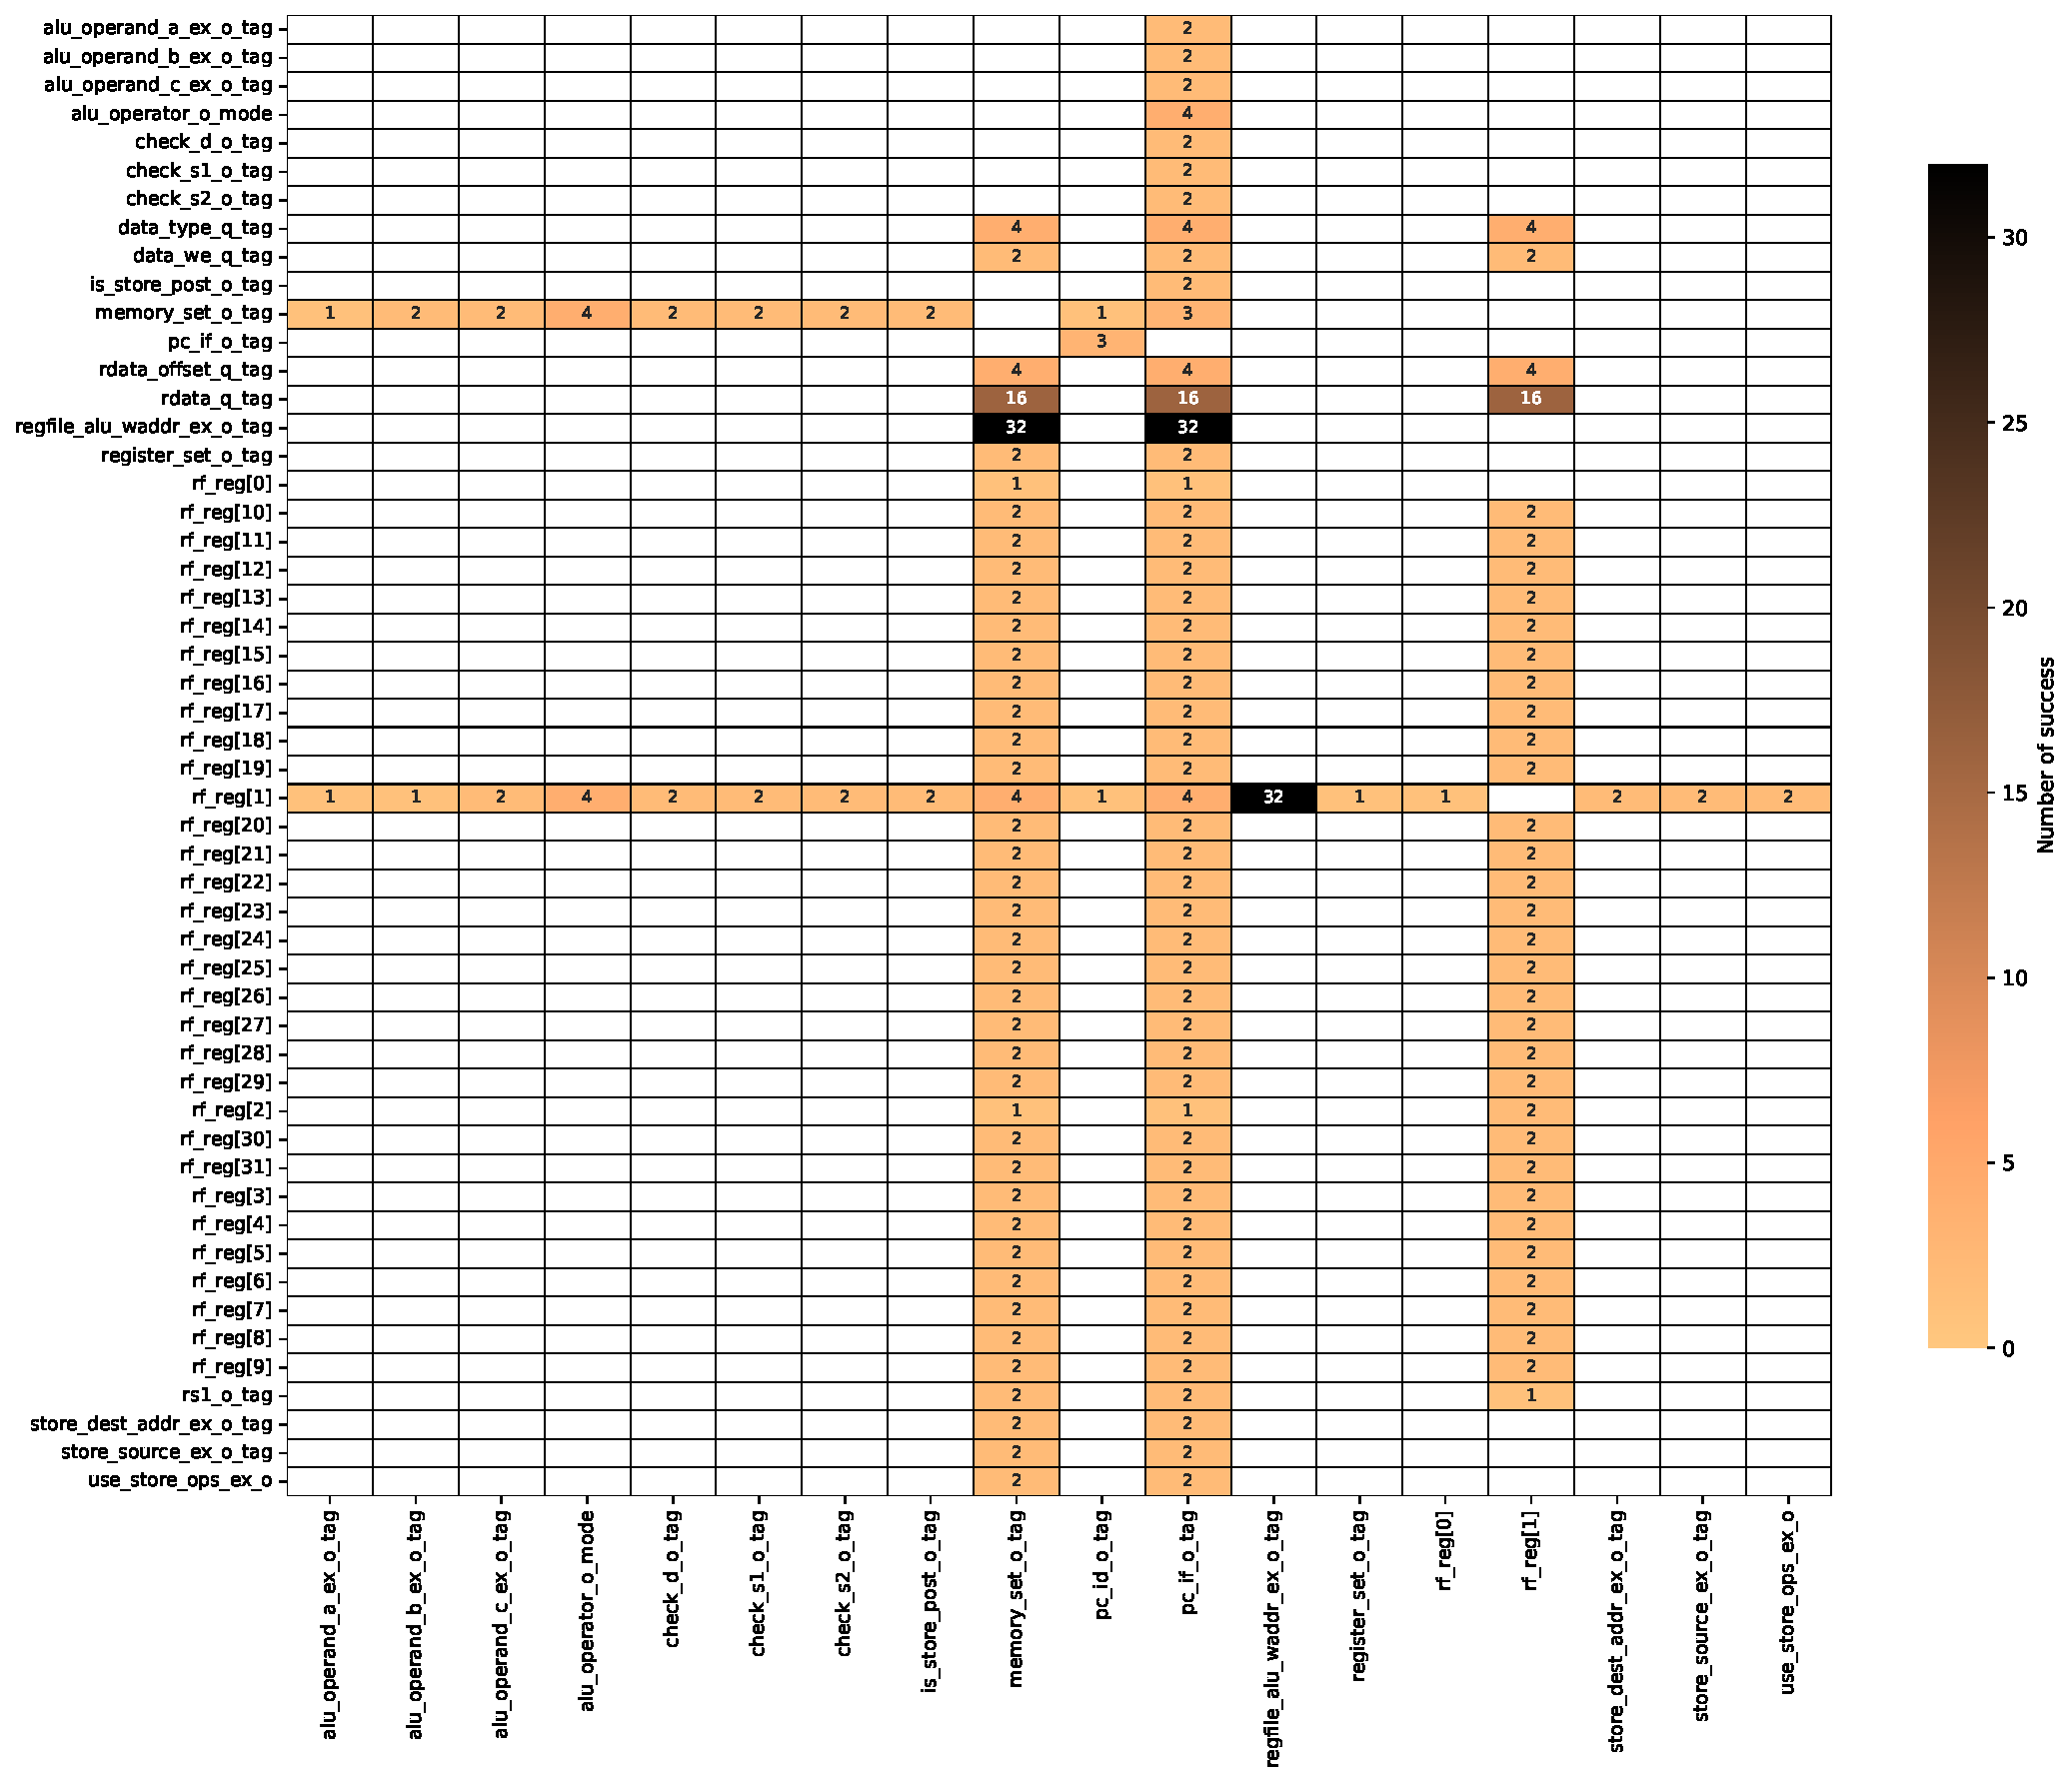
\includegraphics[width=\textwidth]{src/5_results/img/heatmap_buffer_overflow_wop_1_multi_bitflip_reg_multi_2.pdf}
            \caption{Unprotected version: multi-bits faults in two registers at a given clock cycle $\rightarrow$ 450 successes}
            \label{fig:heatmap_multibit_1}
        \end{figure}
    \end{minipage}\hfill%
    \begin{minipage}[c]{0.55\linewidth}
        \only<1>{
            \begin{figure}
                \centering
                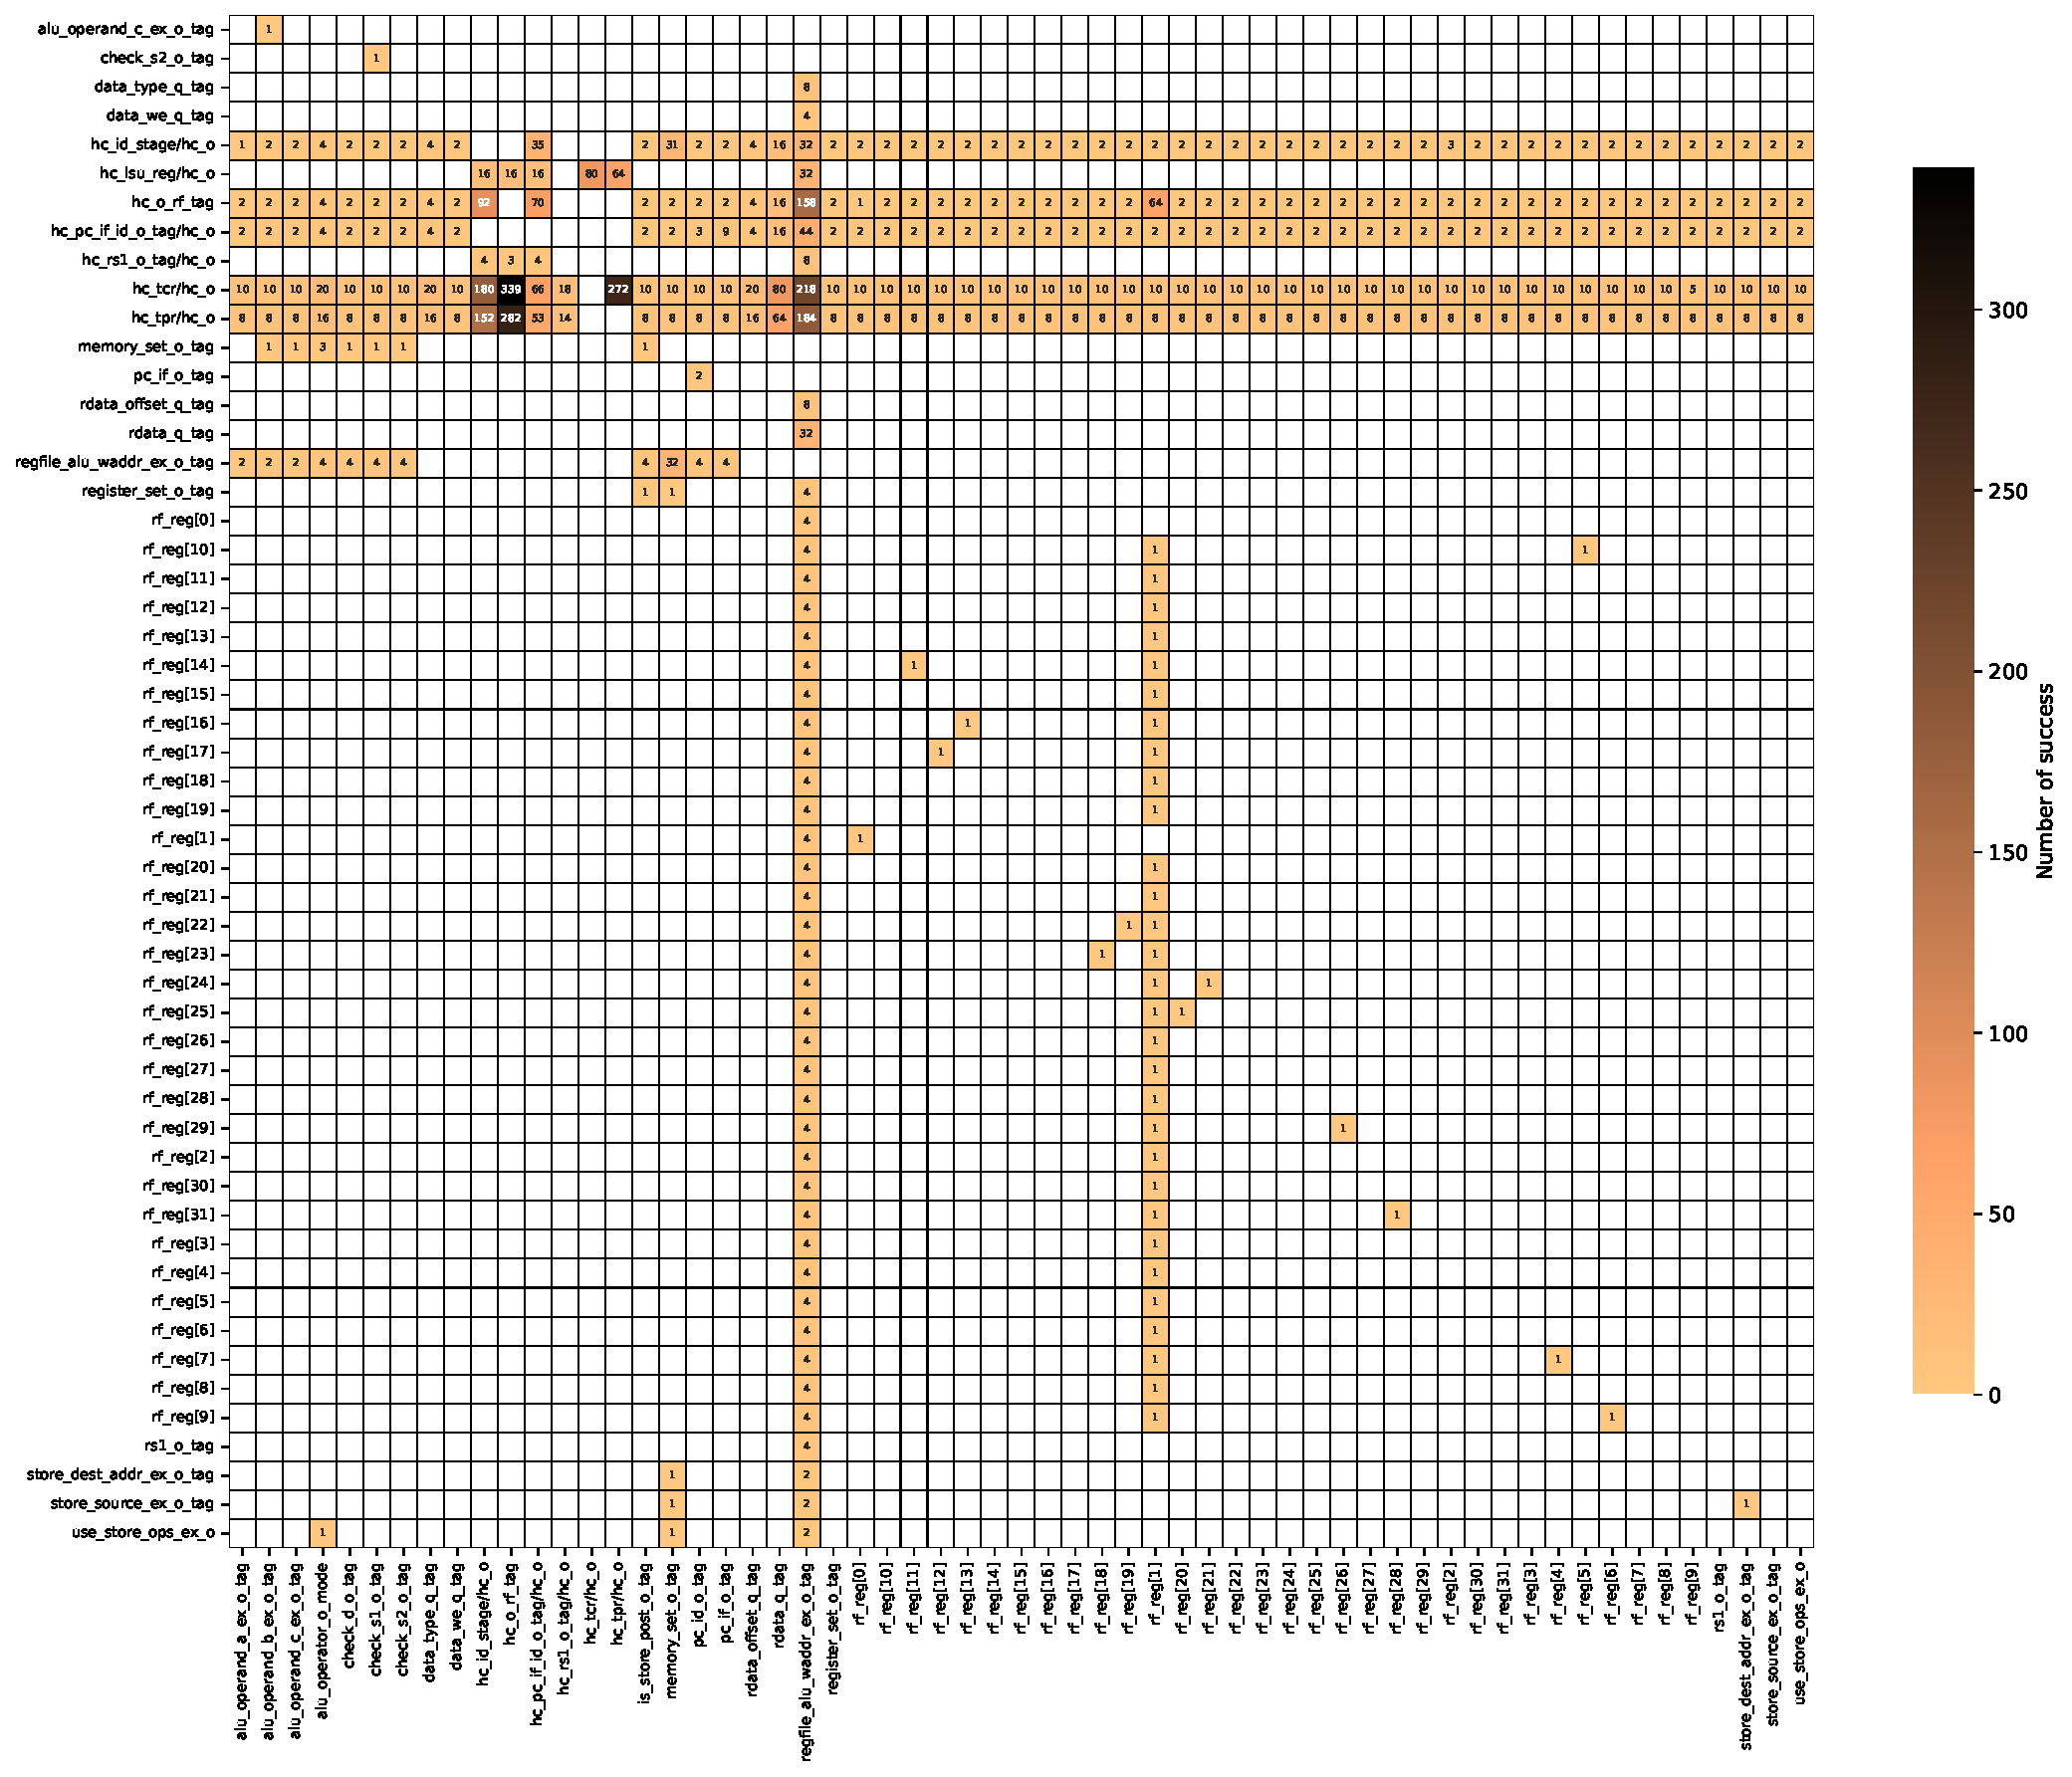
\includegraphics[width=\textwidth]{src/5_results/img/heatmap_buffer_overflow_hamming_2_multi_bitflip_reg_multi_2.pdf}
                \caption{Hamming Code 2 protected version: multi-bits faults in two registers at a given clock cycle $\rightarrow$ 4356 successes}
                \label{fig:heatmap_multibit_2}
            \end{figure}
        }
        \only<2>{
        \begin{figure}
            \centering
            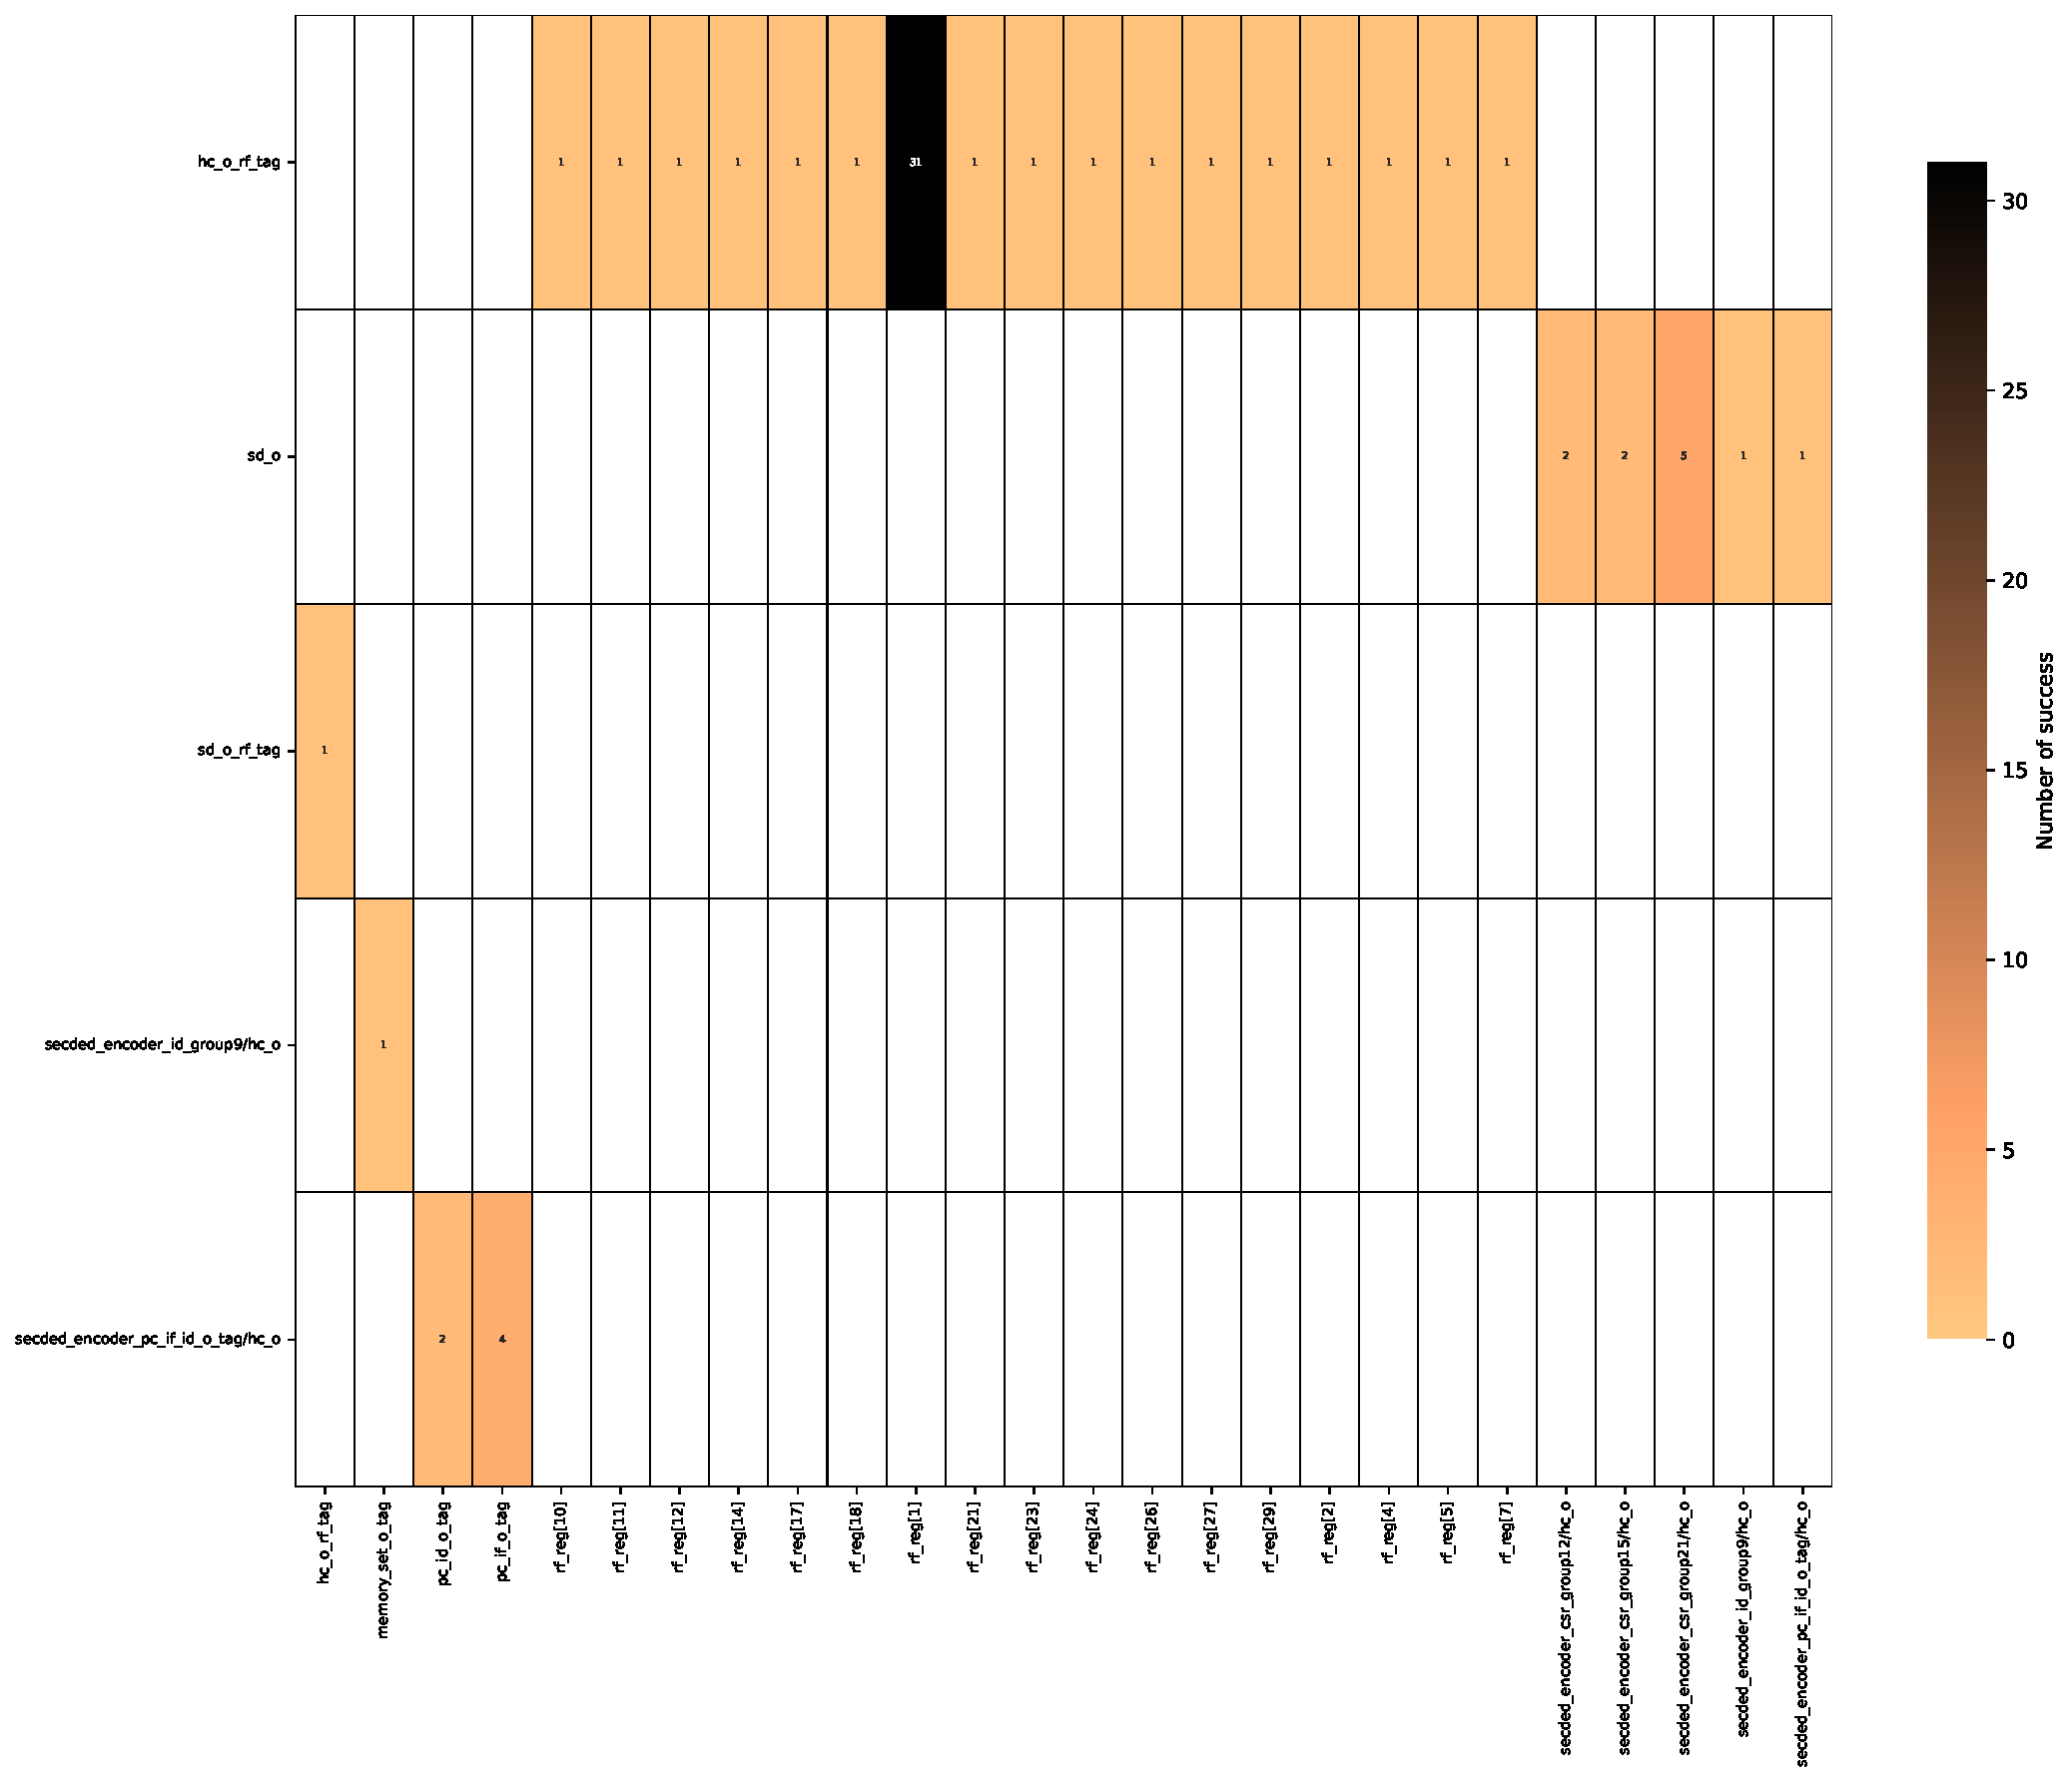
\includegraphics[width=\textwidth]{src/5_results/img/heatmap_buffer_overflow_secded_5_multi_bitflip_reg_multi_2.pdf}
            \caption{SECDED 5 protected version: multi-bits faults in two registers at a given clock cycle $\rightarrow$ 66 successes}
            \label{fig:heatmap_multibit_3}
        \end{figure}
        }
    \end{minipage}
\end{frame}